\documentclass{IOS-Book-Article}
\newif\iflong\longtrue  %toggle longtrue longfalse
% if there is a shorter version, it will have less material
% \iflong
% ... long version material ...
% \fi
\usepackage{mathptmx}
\usepackage{hyperref,url}
\usepackage{graphicx}
\usepackage{float}
\def\Eo{\mbox{\sc Ezo}}
\def\Ec{\mbox{\sc Ezo-CNN}}
\def\Mx{\mbox{\sc MoHex}}
\def\Mc{\mbox{\sc MoHex-CNN}}
\def\Mt{\mbox{\sc MoHex-3HNN}}
\def\Sol{\mbox{\sc Solver}}
\def\Fuego{\mbox{\sc Fuego}}

\def\hb{\hbox to 10.7 cm{}}

\begin{document}
\pagestyle{headings}
\def\thepage{}
\begin{frontmatter}              % The preamble begins here.
%\pretitle{Pretitle}
\title{MoHex3HNN defeats EzoCNN in 2018 Hex tournaments}}

\markboth{}{2018 New Taipei City Computer Games Olympiad Report: to appear in ICGA Journal}
%\markboth{R.~Hayward and N.~Weninger / Hex 2017: \Mx\ wins 11$\times$11 and 13$\times$13 tournaments}
\author{\fnms{Ryan~B.\ } \snm{Hayward}} and
\author{\fnms{Chao} \snm{Gao}%
\thanks{Corresponding author: Ryan~B.~Hayward, UAlberta, Edmonton, Canada,
hayward@ualberta.ca.}} and
\author{\fnms{Kei} \snm{Takada}}%

\runningauthor{AuthorA et al.}
\address{Department of Computing Science, University of Alberta, Canada}
%\address[B]{Department of Computing Science, University of Alberta, Canada}
\end{frontmatter}
\markboth{Hayward, Gao and Takada}{Hex 2018: \Mt\ defeats \Ec}

%\begin{figure}[hbt]
%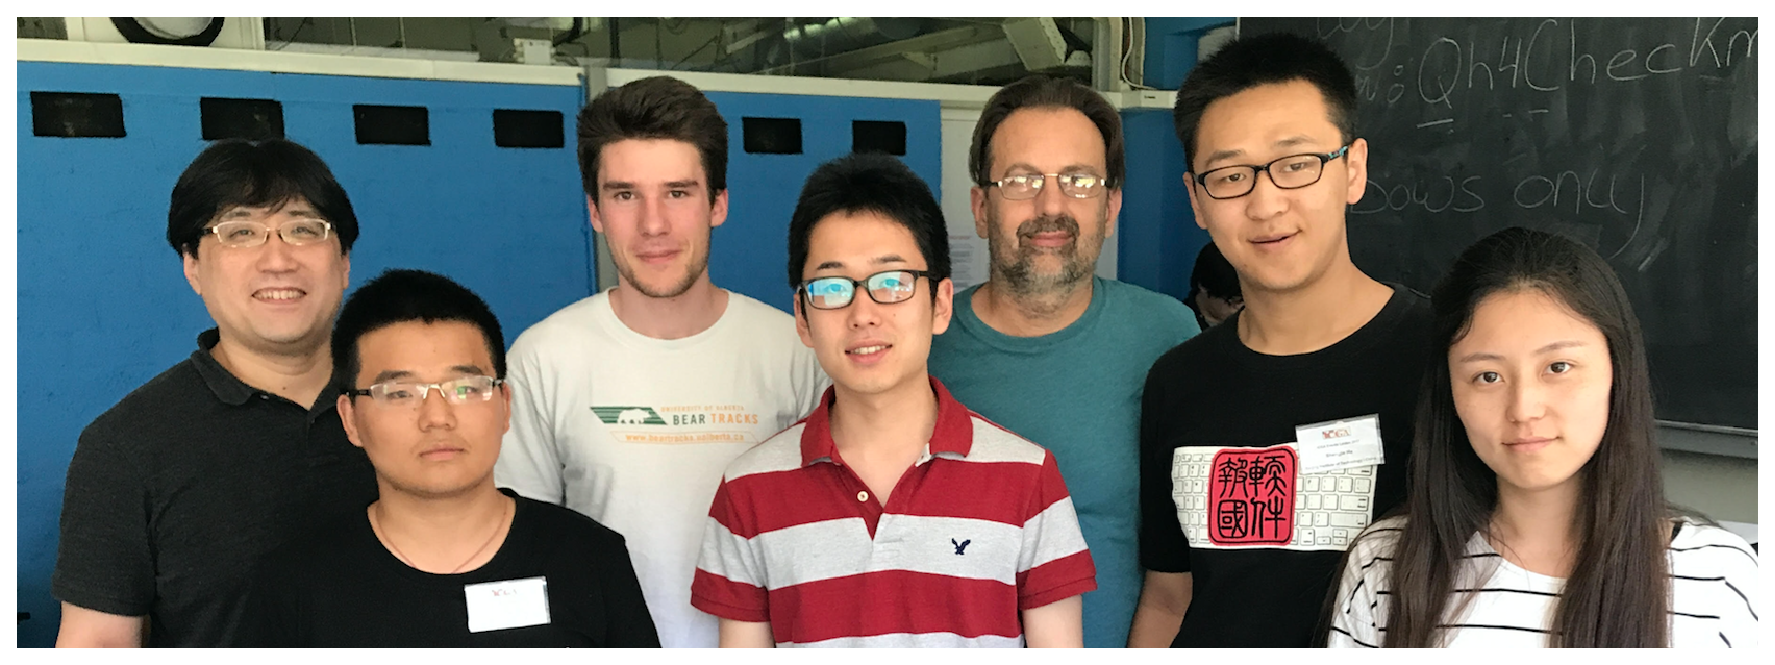
\includegraphics[width=\columnwidth]{photos/people-1.eps}\
%\caption{Participants at the Hex competitions. From left,
%Masahito Yamamoto,
%You RunZe,
%Noah Weninger,
%Kei Takada,
%Ryan Hayward,
%Ma Shengjie,
%Wu Tong.} \end{figure}
%
\section{The Tournaments}
There were two Hex tournaments at the 
2018 Olympiad in New Taipei City:
board-size 11$\times$11 and 
board-size 13$\times$13.\footnote{\cite{H17olyrptsource} has .sgf 
  game records and source files for this report.
  \cite{Hexgui} has an SGF (Smart Game Format) viewer.
  SGF was developed by \cite{SGF}.}
11$\times$11 Hex is the original game introduced by Piet Hein in 1942. 
All one-move openings on all $n$$\times$$n$ Hex boards up to 9$\times$9
have been solved by computers, as have two 10$\times$10 openings 
\cite{PawlH13}.
11$\times$11 games can typically be solved after only 20 to 30 moves
by a computer solver, so in recent years
a tournament on the 13$\times$13 board  ---
a size used by the Little Golem hex community \cite{LittleG} ---
was introduced.

%13 J b2 a3 c12 (b11 a2 c2)
%11 J j2 b4(?) (c2 c10)

Each tournament had the same two contestants:
\Ec{} from Japan, 
by Kei Takada (supervised by Masahito Yamamoto);
and \Mt{} from Canada,
by Chao Gao (supervised by Ryan Hayward and Martin M\"{u}ller),
assisted by 
Jakub Pawlewicz,
Ashley Herman,
Joseph Meleshko,
Jiahao Li,
Paul Banse,
Siqi Yan,
Wai Yi Low
and
Xutong Zhao.
Opening moves were based on self-play game statistics.
The self-play game generation procedure was developed
by Gao and Pawlewicz.

\Mt\ is an AlphaGo-style neural net program that shares
much code from the earlier MoHex 2.0 by 
Broderick Arneson, Philip Henderson, Aja Huang, 
Jakub Pawlewicz, Noah Weninger, Kenny Young and Ryan Hayward.
MoHex versions
won the previous
eight Olympiad Hex competitions \cite{HAHP13},
TODO REF 2017
is an MCTS program that uses the Benzene Hex framework
built on the code base of \Fuego\ \cite{fuego}.
%the Go program developed by Martin M\"{u}ller, Markus Enzenberger
%and others at the University of Alberta.
%Benzene allows virtual connection and
%inferior cell computations.
\Mx{} performs knowledge computation 
in UCT tree nodes visited at least 256 times.
\Mx{} ran on Firecreek, a 24 core shared-memory machine, 
with four cores reserved for the 
DFPNS solver \cite{PawlH13}, which
produces perfect play if it solves the
position within the time allotted.
\Mx{} uses a book built by Broderick Arneson with Thomas Lincke's method 
\cite{DBLP:conf/cg/Lincke00}. 
Noah Weninger expanded the book and added a feature
allowing the use of rotational symmetry for openings
whose rotation is in the book.
For each board size, the book covers at least eight openings.

\Mt{}, the successor of \Mc,
uses a three-head convolutional neural net (CNN)
with 128 filters per layer \cite{ijcai}
and was trained on 400 000 self-play games.
At each new node of the Monte Carlo search tree, 
the three-headed neural net is called
and returns policy, state, and action values.
\Mt{} ran remotely on a machine with four CPU cores and one GPU.

\Eo{}, based on the Benzene framework, 
uses iterative deepening alpha-beta search 
with policy and value functions
learned from 10 000 000 self-play games
generated by minimax search.
\Ec{} ran remotely on a machine
with two CPUs and one GPU.
In some games the internet connection was dropped
and computation restarted on a  laptop.
with one CPU-thread for search and one CPU-thread for
Benzene's Depth-First Proof Number Search endgame solver.

Each tournament was scheduled for 8 games between
each two of the three competitors, with 30'/game per player.
The 13$\times$13 and 11$\times$11 tournaments were played
on July 8 and 9 respectively.


The tournaments started on July 1 and finished on July 5.
See Tables~\ref{tab:tour1} and \ref{tab:tour2} and Figures 2-7.
In many games, the losing operator resigned once Benzene solved the game.
Figures~\ref{fig:EM11} and \ref{fig:EM13} show typical continuations
after resignation.

{\bf Tournament results.}
\Mc\ won the best-of-eight 13$\times$13 competition 5-0
and the 11$\times$11 competition by the same score.

%\begin{figure}
%\hspace*{-2cm}\
%\includegraphics[scale=.9]{pix/11.mh1.eps}\hspace*{-1.5cm}\
%\includegraphics[scale=.9]{pix/11.hm2.eps}\hspace*{-1.5cm}\
%\includegraphics[scale=.9]{pix/11.mh3.eps}\hspace*{-1.5cm}\
%\includegraphics[scale=.9]{pix/11.hm4.eps}
%\caption{\Hite-\Mx\ Games 1-4. M-H 1-0, H-M 0-1, M-H 1-0, H-M 0-1.}
%\end{figure}

\section{11$\times$11 Tournament}
In a game, if the second move is `swap', then players
exchange colors and the first player plays the next move:
in the corresponding diagram, black `S' marks the first two moves
and white `3' the next move.
In the figures, `A-B 1-0' indicates that A plays first, starting as black, 
and A wins (as white if B swapped, as black if not).

%\begin{figure}
%\hspace*{-2cm}\
%\includegraphics[]{pix/11.eh1.eps}\hspace*{-1.5cm}\
%\includegraphics[]{pix/11.he2.eps}\hspace*{-1.5cm}\
%\includegraphics[]{pix/11.eh3.eps}
%\caption{\Hite-\Ec\ Games 1-3. E-H 1-0, H-E 0-1, E-H 1-0.
%In Game 1, Black finishes with one of {\bf \{e8,h7\}}.}
%\end{figure}

%\begin{figure}
%\hspace*{-2cm}\
%\includegraphics[scale=1]{pix/11.em1plus.eps}\hspace*{-1.5cm}\
%\includegraphics[scale=1]{pix/11.me2plus.eps}\hspace*{-1.5cm}\
%\includegraphics[scale=1]{pix/11.em3plus.eps}
%\smallskip
%
%\hspace*{-2cm}\
%\includegraphics[scale=1]{pix/11.me4plus.eps}\hspace*{-1.5cm}\
%\includegraphics[scale=1]{pix/11.me5plus.eps}\hspace*{-1.5cm}\
%\includegraphics[scale=1]{pix/11.em6plus.eps}
%\smallskip
%
%\hspace*{-2cm}\
%\includegraphics[scale=1]{pix/11.me7plus.eps}\hspace*{-1.5cm}\
%\includegraphics[scale=1]{pix/11.em8plus.eps}\hspace*{-1.5cm}\
%\includegraphics[scale=1]{pix/11.em9plus.eps}
%\caption{\Ec-\Mx\ Games.
%a) 1-3. E-M 0-1, M-E 1-0, E-M 1-0.
%b) 4-6. M-E 1-0, M-E 0-1, E-M 1-0.
%c) 7-9. M-E 0-1, E-M 0-1, E-M 0-1.}
%\label{fig:EM11}
%\end{figure}
%
%\begin{figure}
%\hspace*{-2cm}\
%\includegraphics[scale=1]{pix/11.me10plus.eps}\hspace*{-1.5cm}\
%\includegraphics[scale=1]{pix/11.me11plus.eps}\hspace*{-1.5cm}\
%\includegraphics[scale=1]{pix/11.em12plus.eps}
%\caption{\Ec-\Mx\ Games 10-12. M-E 0-1, M-E 1-0, E-M 0-1.}
%\end{figure}
%\iflong
%%This is the longer version, so we include all games.
%%11x11 EM games
 %%1 em 01 a4 s B
 %%2 me 10 g2 s W
 %%3 em 10 h2   B  1st win by Ezo
 %%4 me 10 a2 s W
 %%5 me 01 a6   W
 %%6 em 10 k7 s W
 %%7 me 01 a2   W
 %%8 em 01 k5 s B
 %%9 em 01 k6 s B
%%%10 me 01 a8   W
%
%%{\bf Game 1.} {\sc E-M 0-1.} 1.B[a4] 2.W[swap] \ldots ~ ~ B wins.
%%{\bf Game 2.} {\sc M-E 1-0.} 1.B[g2] 2.W[swap] \ldots ~ ~ W wins.
%%{\bf Game 3.} {\sc E-M 1-0.} 1.B[h2] no swap \ldots ~ ~ B wins.
%%{\bf Game 4.} {\sc M-E 0-1.} 1.B[a2] 2.W[swap] \ldots ~ ~  W wins.
%%{\bf Game 5.} {\sc M-E 0-1.} 1.B[a6] no swap \ldots ~ ~  W wins.
%%{\bf Game 6.} {\sc E-M 1-0.} 1.B[k7] 2.W[swap] \ldots ~ ~ W wins.
%%{\bf Game 7.} {\sc M-E 0-1.} 1.B[a2] no swap \ldots ~ ~  W wins.
%%{\bf Game 8.} {\sc E-M 0-1.} 1.B[k5] 2.W[swap] \ldots ~ ~ B wins.
%%{\bf Playoff Game 1.} {\sc E-M 0-1.} 1.B[k6] 2.W[swap] \ldots ~ ~  B wins.
%%{\bf Playoff Game 2.} {\sc M-E 0-1.} 1.B[a8] no swap \ldots ~ ~  B wins.
%%{\bf Playoff Game 3.} {\sc M-E 1-0.} 1.B[a9] no swap \ldots ~ ~  B wins.
%%{\bf Playoff Game 4.} {\sc E-M 0-1.} 1.B[h2] no swap \ldots ~ ~  W wins.

\section{13$\times$13 Tournament.}
For this tournament no playoff was required.
Again, the final ranking was determined before
all scheduled games had been played,
so the operator of \Ec\  resigned its final games
without play.
%13x13 EM games
%1 me 10 a7    B
%2 em 10 a3 s  W
%3 me 01 a8    W
%4 em 01 d13   W  turned rave back on 
%5 me 10 a3    B
%6 em 01 m6 s  B
%7 me 10 l12 s W
%8 em 01 b5 w  B

%\begin{table}
%\begin{tabular}{|c|c|c|c|c|c|c|}
%\hline {\bf id} & {\bf 13x13} &\Mc{} &\Ec{}  &\Hent{} 
                %& {\bf Total} & {\bf Result} \\ 
%\hline {\bf M} & \Mc{}         &      &  6-2  & 2-0  & 8-2   & gold \\
%\hline {\bf E} & \Ec{}         &  2-6 &       & 4-0  & 6-6   & silver \\
%\hline {\bf H} & \Hent{}       &  0-2 &  0-4  &      & 0-6   & bronze \\
%\hline
%\end{tabular}
%\caption{13$\times$13 tournament results}
%\label{tab:tour2}
%\end{table}

\section{Conclusions}
On 11$\times$11 \Mx\ and \Ec\ seem evenly matched.
\Mx{}'s search seems too narrow, especially near the opening.
In positions with plural good-looking moves,
initial playouts can bias final move selection, and
\Mx\ sometimes makes a bad move early in the game.
The purpose of \Mx's book is to avoid early bad moves.
This played a role in the final playoff game, 
where \Ec{} opened with 1.B[H2].  

%\begin{figure}
%\noindent\hspace*{-2cm}\
%\includegraphics[scale=.9]{pix/13.hm1.eps}\hspace*{-1.8cm}\
%\includegraphics[scale=.9]{pix/13.mh2.eps}\hspace*{-1.8cm}\
%\includegraphics[scale=.9]{pix/13.eh1.eps}
%\smallskip
%
%\noindent\hspace*{-2cm}\
%\includegraphics[scale=.9]{pix/13.he2.eps}\hspace*{-1.8cm}\
%\includegraphics[scale=.9]{pix/13.eh3.eps}\hspace*{-1.8cm}\
%\includegraphics[scale=.9]{pix/13.he4.eps}
%\caption{\Hent{} Games.  a) 1-3. H-M 0-1, M-H 1-0, E-H 1-0.
%b) 4-6. H-E 0-1, E-H 1-0, H-E 0-1.}
%\end{figure}

In an earlier game, \Ec{} played the same opening
and won easily after \Mx\ replied 2.W[f5], 
which is not on the main diagonal and does little to block Black.
But in the playoff game, \Mx\ replied 2.W[g5] and won.
Post-tournament testing shows that \Mx\ likes both moves more than all others,
but that the superiority of {\bf g5} to {\bf f5} is not clear.
If initial rollouts are unlucky, \Mx\ will not see that {\bf g5} is better.

On 13$\times$13 \Mc\ seems stronger than \Ec.
\Mc\ suffered from a lack of testing prior to the tournament.
Consequently, it played the first three games with 
its rapid access value estimation (RAVE)
feature turned off. This search was too narrow, 
so RAVE was turned on for the remaining five games, which improved
performance.

\begin{figure}
\noindent\hspace*{-2cm}\
\includegraphics[scale=.9]{pix/13.me1plus.eps}\hspace*{-1.8cm}\
\includegraphics[scale=.9]{pix/13.em2plus.eps}\hspace*{-1.8cm}\
\includegraphics[scale=.9]{pix/13.me3plus.eps}
\smallskip

\noindent\hspace*{-2cm}\
\includegraphics[scale=.9]{pix/13.em4plus.eps}\hspace*{-1.8cm}\
\includegraphics[scale=.9]{pix/13.me5plus.eps}\hspace*{-1.8cm}\
\includegraphics[scale=.9]{pix/13.em6plus.eps}\
\smallskip

\noindent\hspace*{-.4cm}\
\includegraphics[scale=.9]{pix/13.me7plus.eps}\hspace*{-1.8cm}\
\includegraphics[scale=.9]{pix/13.em8plus.eps}
\caption{\Ec{}-\Mc\ Games. 
a) 1-3. M-E 1-0, E-M 1-0, M-E 0-1.
b) 4-6. E-M 0-1, M-E 1-0, E-M 0-1.
c) 7-8. M-E 1-0, E-M 0-1.}
\label{fig:EM13}
\end{figure}
%\fi

\section*{Acknowledgements}
We thank the NSERC Discovery Grant Program for research funding.
\bibliographystyle{plain}
\bibliography{rpt}
\end{document}
